% !Mode:: "TeX:UTF-8"
\chapter{限制分支预测宽度的改进策略}

本章首先介绍香山第一版架构的取指策略,接下来接受为什么需要限制分支预测的宽度,过宽的分支预测宽度会对整体设计带来怎样的影响。最后介绍FTB相关的功能和实现,具体有FTB表项的数据结构设计,以及FTB更新和管理策略,并解释了为什么要这样设计。通过修改每拍取指的基本单位,实现了限制前端在一次取指内容中分支指令的上限。

\section{香山第一版取指策略}

在香山第一版的设计中,取指pc是按照32Bytes对齐的,也就是低5位都为0,然后每次取指固定取32Bytes的指令数据。这样做的好处首先在于可以有效避免一次取指需要的指令跨Cache行的情况,取指单元在每次取指只需要访问一个Cache行。而这一点在第二版的设计中修改了,因此第二版的取指单元在每次取指时最多可以同时取上来2个Cache行的数据。其次就是由于指令都是对齐的,因此一条指令在整个取指的packet中的位置是固定的,由低5位决定。这样可以保证在进行分支预测时,每条分支指令都只会被预测器的同一个bank预测、记录和更新,不会出现同一条指令在不同bank的情况。而第二版的设计中的取指不再对齐,也因此有可能出现同一条分支指令保存在不同的表项中的情况,这在某种程度上会降低预测器存储空间的使用效率。

但是按照32Byte对齐取指也有一些弊端,首先就是如果某次取指的起始pc非常靠近它所在的Cache行的末尾,由于取指单元不能够跨Cache 行取指,那么这次取回的有效指令数量就不满32Byte,一定程度上会降低取指的带宽。其次也是决定在第二版中修改这个机制的最主要的原因,就是由于香山实现了RISC-V的C扩展,即压缩指令集,RISC-V正常的一条指令 (RVI) 占4个Bytes,而C扩展中规定了许多压缩指令 (RVC),这些压缩指令只有2个Bytes长。增加了压缩指令之后,会带来一些问题,首先就是即使取指是按照32Byte对齐的,但是仍然会出现需要跨行取指的情况,如图\ref{fig:figure31}所示,为了便于表示,以一个cache行 8Bytes为例,当然实际设计中一个cache行会大得多。图\ref{fig:figure31}(a)是不带压缩指令的情况,所有指令都是对齐的,不会出现一条指令在两个cache行中各存一半的现象,但是加入了压缩指令之后就会出现图\ref{fig:figure31}(b)的这种情况,即由于加入了压缩指令,非压缩的指令无法对齐,就会出现一条非压缩指令被2个相邻的cache行截断的情况。

\begin{figure}[htb]
    \centering
    \setlength\tabcolsep{3pt}  % 同一行中的图片间隔
    \vspace{5pt} % 图片上部的空白,如果太小的话,图片顶部会与正文内容十分接近
    \begin{tabular}{ccc}
        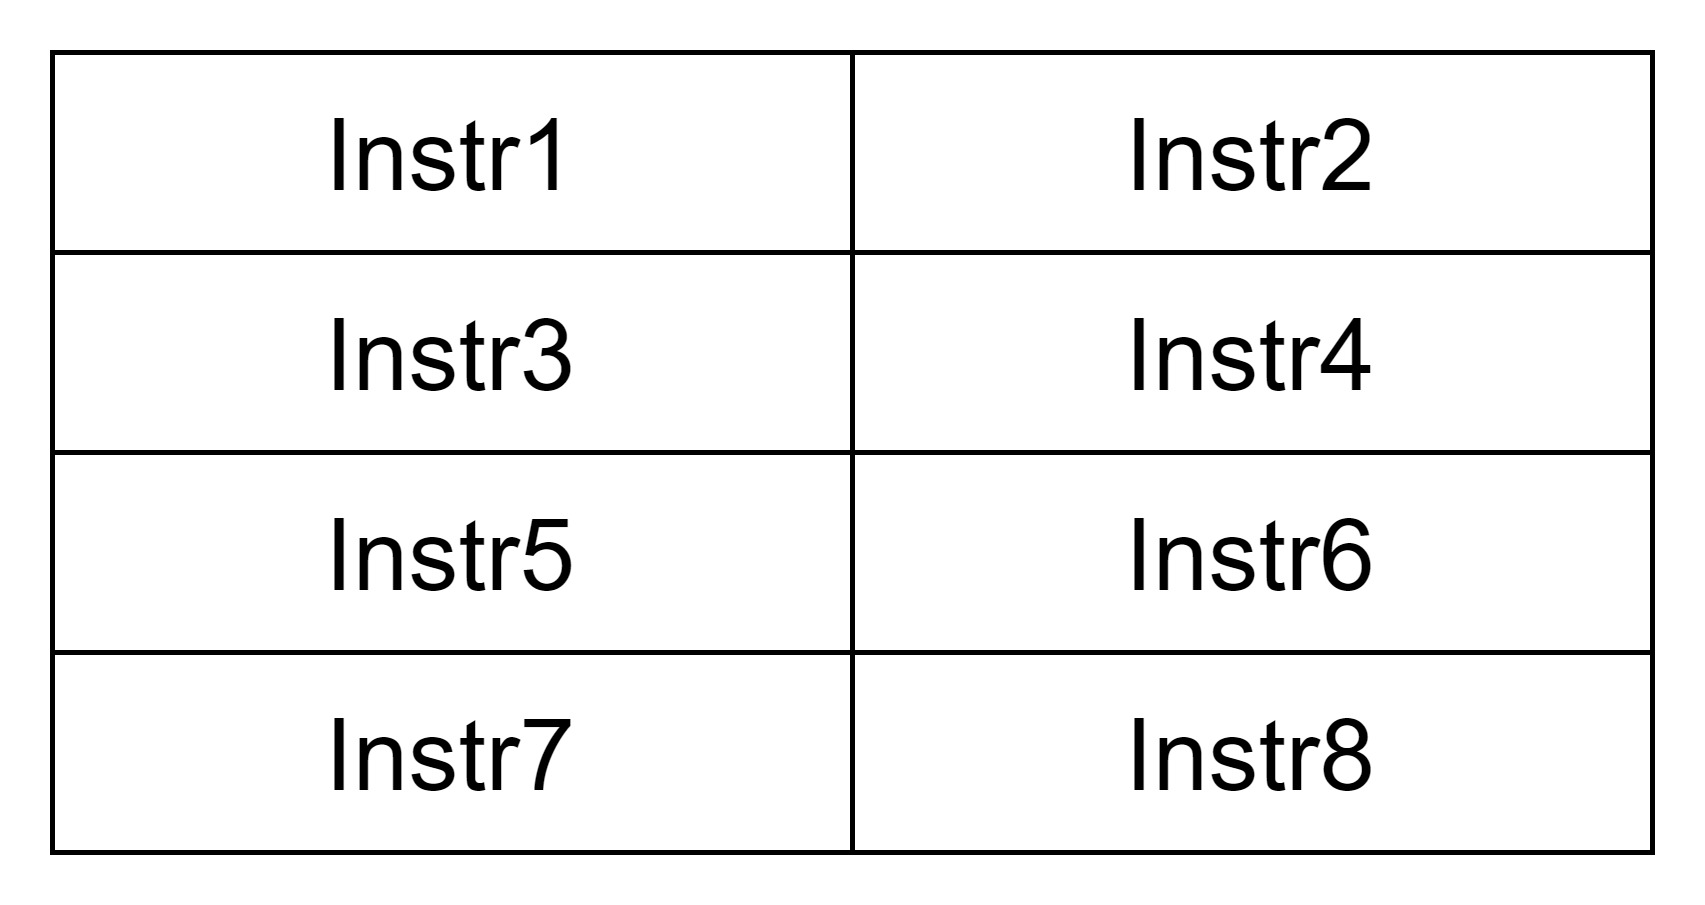
\includegraphics[width=0.30\textwidth]{RVI-only.jpg} &
        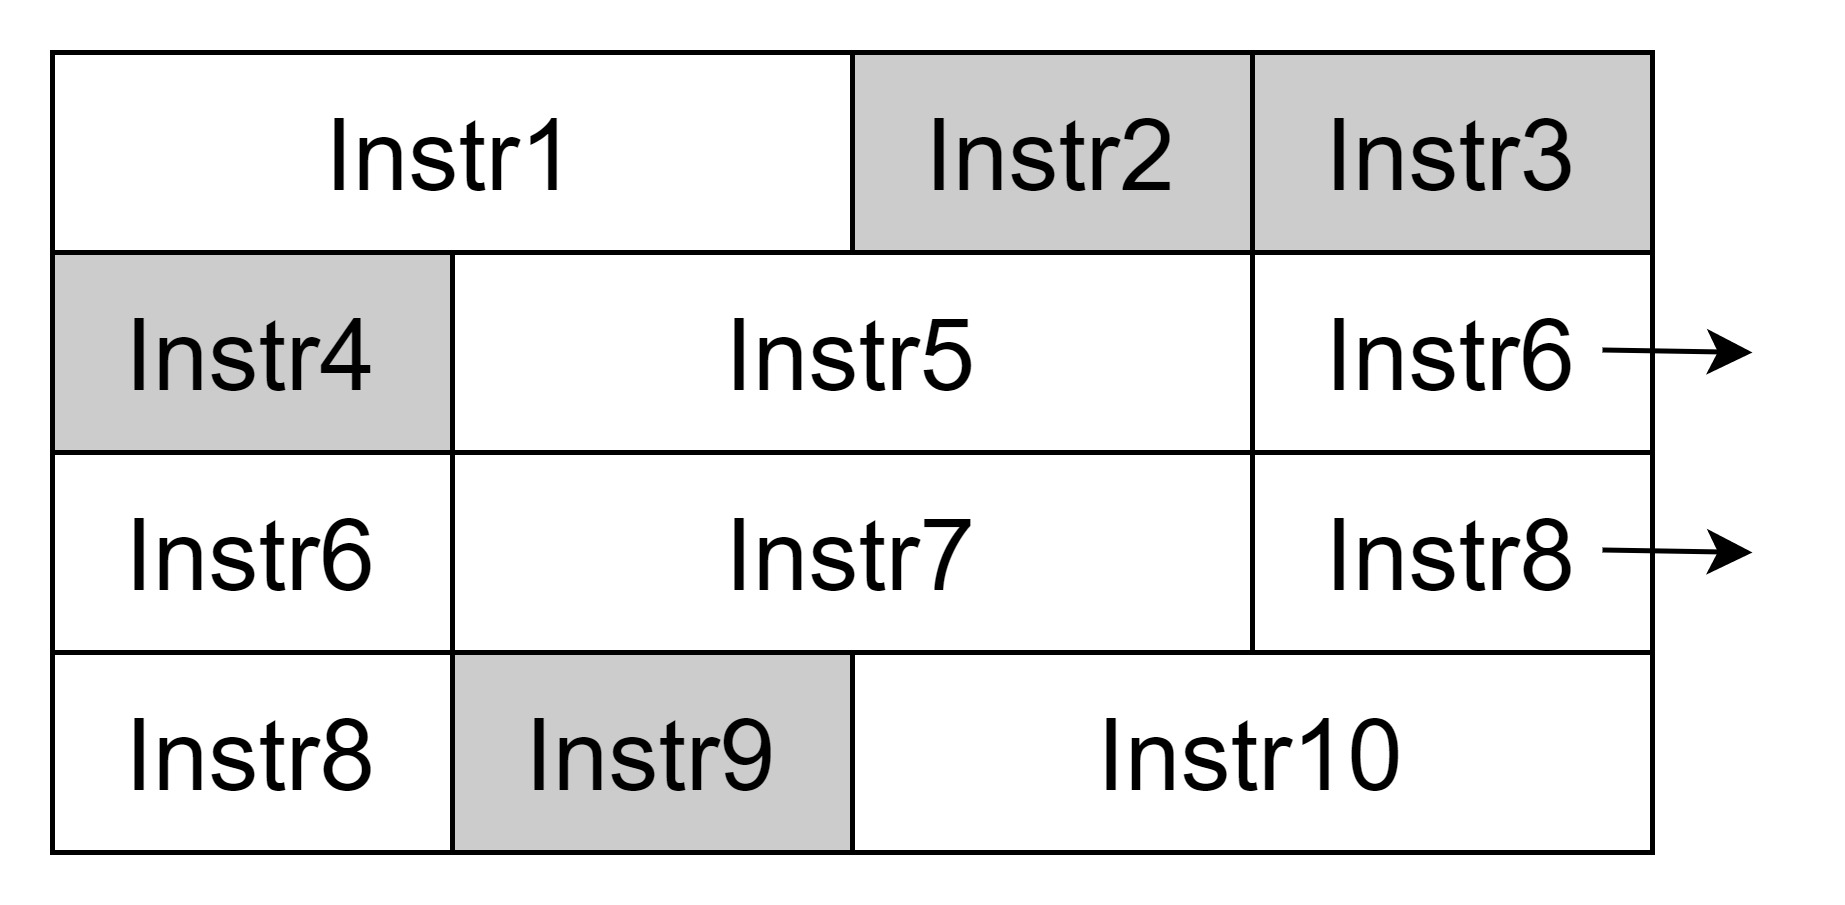
\includegraphics[width=0.325\textwidth]{RVIC.jpg} &
        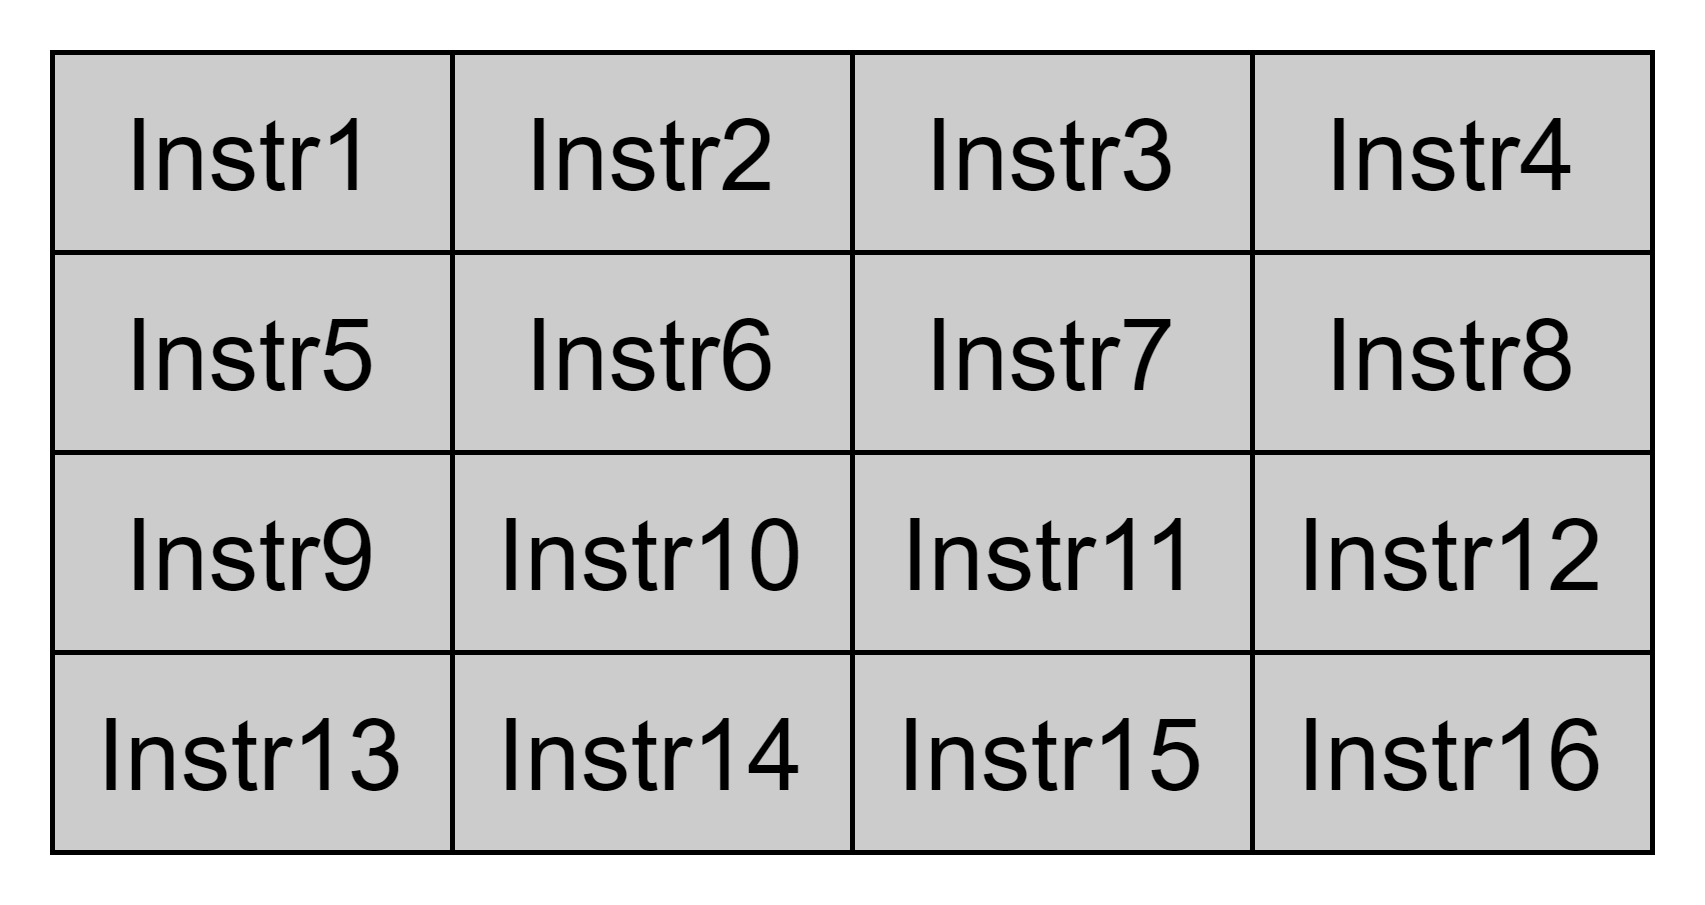
\includegraphics[width=0.30\textwidth]{RVC-only.jpg} \\
        (a) 只有RVI指令 & (b) RVI,RVC指令混合 & (c) 只有RVC指令 \\[1ex]
    \end{tabular}
    \caption{在cache行中以不同形式储存的指令码,其中白色的代表非压缩指令RVI,灰色的代表压缩指令RVC,图(b)中第6和第8条指令跨cache行了}
    \label{fig:figure31}
\end{figure}

当出现这种情况时,就会导致最后这条分支指令无法在一个周期内被完整取出,如果这条被截断的指令正好是条分支,也只有等到下一周期取到后半条指令码后才能对它进行预译码操作。

加入了压缩指令之后,如果以32Byte为单位取指,每次取出来的数据中会有8到16条指令不等,最多的情况如图\ref{fig:figure31}(c)所示,即16条都是压缩指令的情况。因此为了能够覆盖到所有情况,香山第一版的分支预测设计中,所有的预测器,包括第一版中FTB的原型BTB (Branch Barget Buffer) 都是以16为宽度来设计的,也就是说每个预测器都有16个bank,每个bank对应32Bytes中所有有可能是一条分支的位置。

但是实际上真正在程序运行中,一次取出的指令里有这么多条分支指令的情况非常少见,这种设计在一定程度上是冗余的,意味着所有的分支预测逻辑的连线和复杂度都会大大增加,尤其是在分支预测决定最终的预测结果,给出下一周期需要预测的pc的时候,需要从预测器16个bank的预测结果中选出一条最终预测跳转的分支,从16个备选的跳转目标地址中选出一个最终的地址,这是一个4级的多选操作,而这个逻辑处于整个分支预测的关键路径上,许多的组合逻辑电路都要经过这段逻辑,因此降低分支预测宽度,能够减少分支预测的组合逻辑复杂度,减少选择最终预测结果的逻辑门数,如图\ref{fig:figure33}所示,最终达到优化时序,提高频率的效果。

\begin{figure}[htb]
	\centering
	\setlength\tabcolsep{3pt}  % 同一行中的图片间隔
	\vspace{5pt} % 图片上部的空白,如果太小的话,图片顶部会与正文内容十分接近
	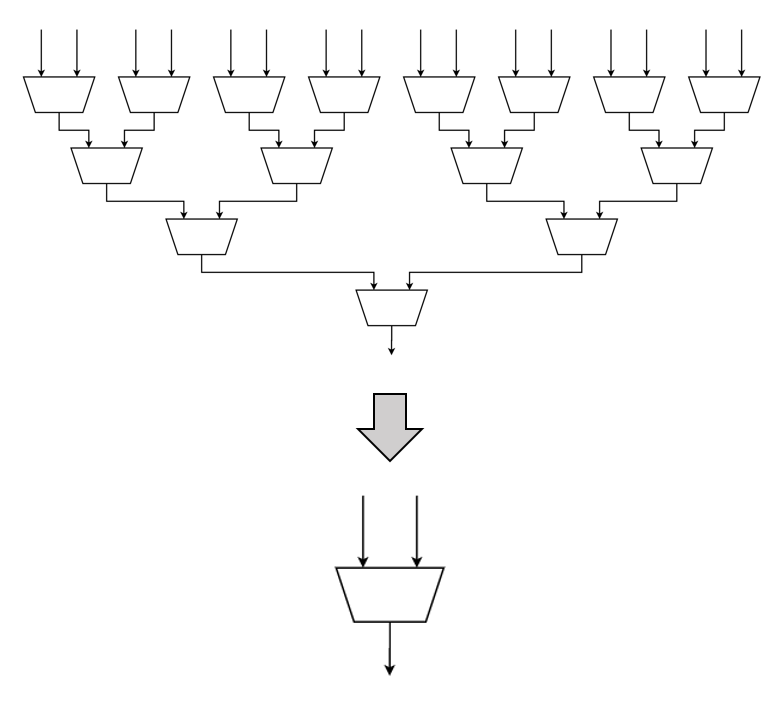
\includegraphics[width=0.7\textwidth]{mux.png}
	\caption{降低分支预测宽度后,选择最终生效分支指令的选择逻辑门层数变少}
	\label{fig:figure33}
\end{figure}

\section{Fetch Block的定义}

为了降低分支预测宽度,一个思路就是限制每次取指所能包含的分支指令的最大数量,因为分支预测最终的宽度是以可能的最大分支数量为准的,例如上文提到的如果一次最多会有16条分支,那么分支预测宽度也必须为16,即使大部分时候并没有这么多分支。
假设将分支预测的宽度限制为2,之前的取指是以32Byte定长为单位取指的,而在一些分支指令密集的程序片段中,32Bytes大小的指令块中很大概率会出现超过2条分支,因此不能够继续以固定的大小作为取指的基本单位,需要定义一个新的基本单位,为这个单位添加一些约束条件,以此来限制每次取指的分支指令数量。

在第二版的分支预测架构中,定义了Fetch Block,这个概念是Glenn\cite{scalable-frontend}提出的,Fetch Block的定义如下,每个block都必须满足这三个约束条件:

\begin{enumerate}
    \item 每个block的最大大小为32Byte,即当一段指令中没有分支指令时,仍然需要限制block的最大大小,因此规定block的最大大小和第一版架构相同,都是32Byte。
    \item 当遇到第n+1条条件跳转指令 (branch) 时,无论block大小有没有32Byte,这个block在第n+1条branch指令之前截止。为什么不是在第n条指令后就立即截止,是因为这样就可以保证,在block中最多只有n条分支的前提下,每个block中的指令数量尽可能多。
    \item 当遇到无条件跳转指令 (jump) 时,无论block大小有没有32Byte或有没有达到n条branch指令的上限,这个block都在这条jump指令后截止。这是因为jump指令必然是跳转的,因此在这条指令之后下一周期需要预测的pc应该由预测器给出,无论下一周期从哪里开始预测,都将会是另一个block。因此如果block中含有jump指令,必定是block中最后一条指令。
\end{enumerate}

通过以上的3条约束,就能够保证单个的Fetch Block中,branch指令不超过n条,且最多只有一条jump指令。而在此基础上,又提出了一种改进策略,可以略微减少FTB表项的大小,节省一些面积。可以将每个block中看作有n个装branch指令的slot和一个装jump指令的slot,假设因为遇到第n+1条指令导致block截止时,其中存储jump的slot就被闲置了;而遇到jump指令,且之前不足n条branch指令时,第n条branch指令的slot也被闲置了,而这两种情况非常常见,带来了空间的浪费。针对这种现象做出了改进,即令第n条branch指令与jump指令共用一个slot,也就是在block中的最后一个slot既可以用于存储一条branch指令的信息,也可以用于存储一条jump指令的信息。这样一个block中就变为最多可以同时有n条branch指令,或者同时有n-1条branch指令和1条jump指令。

通过Fetch Block的定义不难发现,Fetch Block是不可能按照地址对齐的。因此同一条分支存在于两个不同的Fetch Block中是有可能的,而这种情况会带来一定的存储空间浪费,经过测试,在使用相同SRAM开销的情况下,以Fetch Block为表项存储FTB的命中率是略低于以分支指令为表项存储的BTB的命中率的。因此第二版中增加了FTB使用的STAM大小。另外一个block中的指令跨Cache行也是有很大概率出现的情况,因此在第二版的设计中,取指单元每次取指可以取出两个Cache行,以保证每个block都能在一次指令缓存访问中取出。

\section{FTB的数据结构设计}

% 投稿论文的主要内容

为了在硬件中实现以Fetch Block为表项的FTB,设计了一种FTB表项的数据结构,相关的属性以及作用在表\ref{tb:table1}中列出。通过这些属性,就能够清楚的描述一个Fetch Block的状态,以及其中含有的分支指令的相关信息。

\begin{table}[]
	\caption{FTB表项属性列表}
	\label{tb:table1}
	\centering
	\begin{tabular}{|c|c|c|}
		\hline
		属性名   & 数据类型   & 含义及作用   \\ \hline
		valid & Bool & 代表这个表项是否有效 \\ \hline
		tag & Unsigned Int & Fetch Block起始地址的高位 \\ \hline
		brSlots & Vector(FtbSlot) & 用来存储branch指令的信息,FtbSlot的定义见表\ref{tb:table2} \\ \hline
		tailSLot & FtbSlot & 用来存储branch/jump指令的信息 \\ \hline
		pftAddr & Unsigned Int & \tabincell{c}{代表这个block最后一条指令的下一条指令的起始pc, \\ 存储低位,使用拼位计算} \\ \hline
		carry & Bool & 代表拼位计算时高位要不要加1 \\ \hline
		isCall & Bool & 如果block中有jump时,代表这条jump是否是call指令 \\ \hline
		isRet & Bool & 如果block中有jump时,代表这条jump是否是ret指令 \\ \hline
		isJalr & Bool & 如果block中有jump时,代表这条jump是否是jalr指令 \\ \hline
		last\_may\_be\_rvi\_call & Bool & 最后一条指令可能是半条RVI Call指令 \\ \hline
		always\_taken & Vector(Bool) & 这条指令是否总是跳转 \\ \hline
	\end{tabular}
\end{table}

从表\ref{tb:table1}中可以看出,在FTB表项中,存储了Fetch Block的tag、分支指令的相关信息,以及计算Fetch Block结束地址的相关信息。其中的brSLots和tailSlot是用来存储block中的branch和jump指令信息的,它们是同一种数据结构FtbSlot,不同之处在于brSlots是一个有n个FtbSlot的列表,而tailSlot就是一个单独的FtbSlot。FtbSlot的相关属性以及作用在表\ref{tb:table2}中列出。

\begin{table}[]
	\caption{FtbSlot属性列表}
	\label{tb:table2}
	\centering
	\begin{tabular}{|c|c|c|}
		\hline
		属性名   & 数据类型   & 含义及作用   \\ \hline
		valid & Bool & 这条branch/jump是否有效 \\ \hline
		offset & Unsigned Int & 这条branch/jump指令在block中的offset \\ \hline
		lower & Unsigned Int & \tabincell{c}{这条branch/jump的target的低位, \\ branch和jump的offset length是不同的} \\ \hline
		tarStat & Unsigned Int & \tabincell{c}{这条branch/jump指令的目标地址高位是需要加1或者减1或者不变, \\ 0代表不变,1代表加1,2代表减1} \\ \hline
		sharing & Bool & 这个slot现在存的是一个branch还是一个jump \\ \hline
	\end{tabular}
\end{table}

一个Fetch Block的起始地址就是block中第一条指令的pc,而block的结束地址应该是block中最后一条指令的pc。但是由于指令分为4Byte的RVI指令和2Byte的RVC指令,所以如果存储block中最后一条指令的pc,并不知道最后一条指令的长度是4Byte还是2Byte,就无法推断出这个Fetch Block后面连续的Fetch Block的起始地址,因此需要存储下一个顺序Fetch Block的起始地址,称为fallthrough address。而完整的fallthrough address可以通过起始地址和pftAddr (partial fallthrough address) 以及carry属性计算得到。由于一个Fetch Block最大的大小不超过32Byte,以香山举例,完整的指令地址有39位,通常来说一个Fetch Block的起始地址和结束地址的高34位要么是相同的,要么结束地址的高34位是起始地址的高34位加1。因此没有必要存储完整的fallthrough address,只需要存储fallthrough address的低5位,以及它的高位是否需要由起始地址加1得到即可,在计算fallthrough address时只需要使用block起始地址的高34位+ carry,再与pftAddr拼接,即可得到39位的完整fallthrough address。

而FtbSlot中的lower和tarStat类似于pftAddr和carry,不同之处在于分支指令的跳转距离不止32Byte,因此lower的位数等于指令码中用于计算偏移地址的offset字段的位数,且由于jump指令的offset字段和branch指令的offset字段位宽不同,因此brSlots和tialSlot中lower的位宽也不同。同时由于分支指令既可以向前跳转,又可以向后跳转,因此分支指令的跳转目标地址高位有3种可能:与block的起始地址相同、起始地址加1、起始地址减1。所以tarStat需要2bit位宽,可以表示0、1、-1三种情况。需要计算某条分支的跳转目标地址时,也是将起始地址的高位加上tarStat,再与lower拼接得到完整的目标地址。

isCall和isRet属性主要用于标记哪些分支需要使用RAS进行预测。isJalr用于标记哪些分支是间接跳转分支指令,需要使用ITTAGE预测器预测。

always\_taken是对于一些固定跳转分支的优化,一条分支只有在至少一次跳转之后,才会被认作有效的分支加入FTB中,而一条刚加入FTB的分支会为它标记为always taken,之后无论预测器预测结果如何,都会预测这条分支是跳转的,如果这条分支之后有一次不跳转,always taken标志就会被消除。

\section{FTB的管理策略}

在第一版架构BTB设计中,每次有指令提交后,如果其中有分支指令,就会在BTB中找到分支指令pc对应的表项,选择一个空闲的way写入,如果所有的way都已经被占用,就使用随机替换方式,替换已有的一个表项。而由于在第二版的架构中使用了以Fetch Block为基本单位的FTB,并且计划将其替换策略更改为plru算法,因此FTB的管理策略有较大的改动。

在FTB的设计中,由于限制了每个Fetch Block中分支指令的最大数量,因此大部分时候一个block中的有效数据是小于32Byte的,这一定程度上会导致FTB的存储空间使用效率不高。所以,为了尽可能增大每个Fetch Block中有效指令的数量,在新建Fetch Block时先将所有未跳转过的分支指令都看作普通的指令,只有跳转过的分支才会被记录到FTB中,而实际上,在程序中,一些一直不跳转的分支指令也占有一定的比例,这样就可以直接忽略这类分支指令。而这种策略就导致了随着越来越多的分支指令跳转之后,每个fetch block的大小,其中分支指令的分布情况,在程序执行过程中是动态改变的,因此需要有一个完善的策略,针对不同的情况对FTB中的相关信息进行维护。

经过分析可以将FTB表项的更新分为以下几种情况:

\begin{enumerate}
	\item 在最开始时,FTB为空,因此所有的分支指令都识别不出来,默认都是不跳转,所以最初的所有Fetch Block都是32Byte,且其中视为没有任何分支指令。
	\item 在一次指令提交中,原有的block中检测到了新的branch指令,而block中的branch指令数量没有达到上限,还有多余的slot时,将新的branch指令插入到这个block中。
	\item 在一次指令提交中,有新的branch指令加入,但block中已经没有多余的slot时,需要对比新的branch指令和block中已有branch指令的先后关系,取前n条branch指令按顺序加入到block中,n代表当前block中所能够存储的branch指令的最大值。剩余的一条branch指令需要从block中去除。
	\item jump指令不存在不跳转的情况,因此一定是在新建block的时候加入到存放jump的slot中,而如果是共享slot的话,如果有新的branch指令,它的pc在jump指令之前,就需要将jump挤出该block,branch指令存入共享的slot中,这条jump指令之后会被加入到一个新建的block中。
\end{enumerate}

% 这里的逻辑有空再理一理

无论是上面的哪一种情况,除了需要根据不同的情况调整slot中的数据,由于最后一条分支可能会改变,因此还需要修改block的fallthrough address。图\ref{fig:figure32}画出了不同情况下需要做的操作。首先需要看这条新的branch指令能否插入到block中,如果不能,说明所有的slot都满了,且它们的指令序都在这条新的branch指令之前,所以根据Fetch Block的定义,block在第n+1条branch指令之前截止,且这条指令的pc和block的起始地址之间不超过32Byte的大小要求,则需要将fallthrough address修改为这条新的branch指令的pc。而如果这条branch指令能够插入,且没有分支指令被替换出block,则fallthrough address可以保持不变。如果有分支指令被替换出block,无论是branch指令还是jump指令,都将fallthrough address设为被替换出block的指令的pc。

\begin{figure}[htb]
	\centering
	\setlength\tabcolsep{3pt}  % 同一行中的图片间隔
	\vspace{5pt} % 图片上部的空白,如果太小的话,图片顶部会与正文内容十分接近
	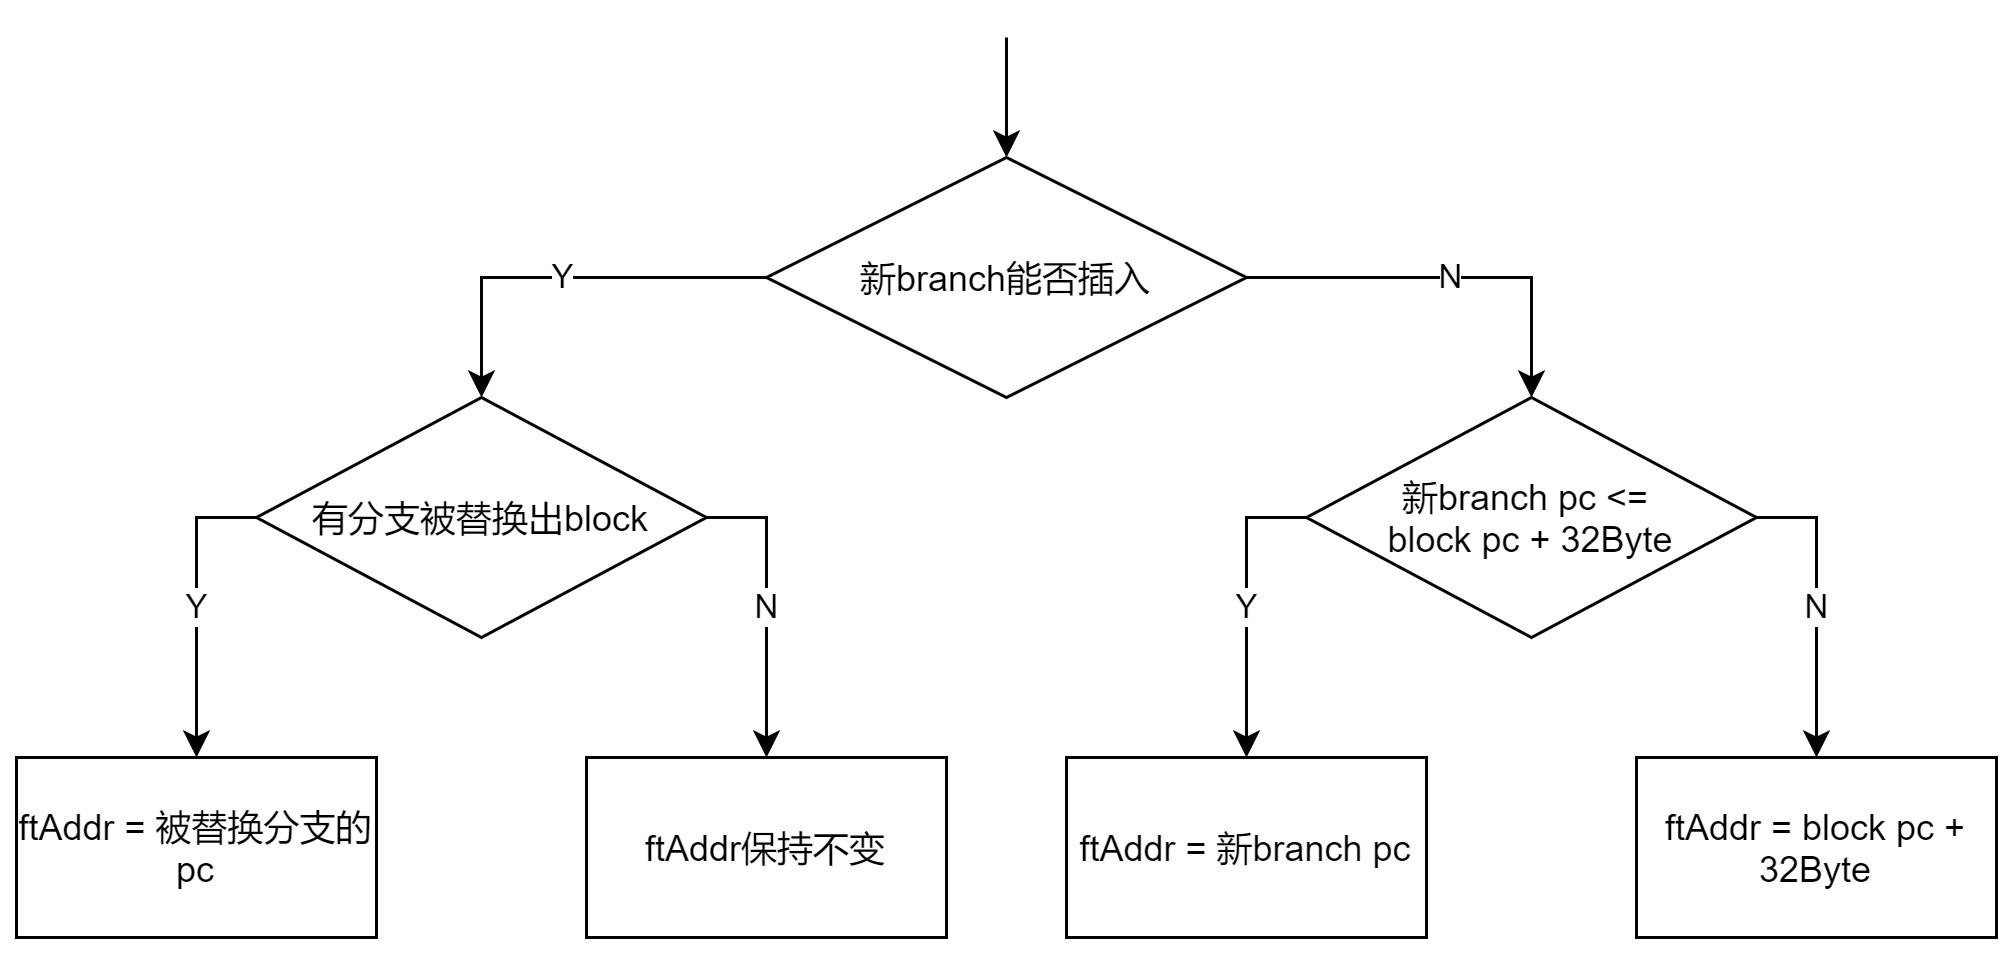
\includegraphics[width=1\textwidth]{ftb-manage.jpg}
	\caption{FTB更新时Fetch Block fallthrought address的变化,ftAddr表示fallthrough address}
	\label{fig:figure32}
\end{figure}

除了维护已有的Fetch Block,如果有新的block需要写入FTB,但是对应的way已经满了,就需要选择其中一个block替换出去,在第一版的架构中BTB使用的是随机替换策略,在第二版中改为了PLRU替换策略,并且使用的是用Chisel实现的通用替换策略模块,可以非常快速灵活的更改替换策略,香山的各级缓存中使用的也是相同模块。

在写入新的block时需要注意,如果这个block已经在FTB中存在了,那么只需要更新其中的block即可,而不能够写入两个起始地址相同的block,这样会导致查找FTB时出现多路命中 (multiple hit) 的错误,这会影响到FTB中存储信息的正确性,从而影响分支预测的性能。因此,在添加或者替换block之前,首先需要确认这个block是否已经存在于FTB之中。最直观的方法就是查找一次FTB,就可以知道block是否已经存在了,但是由于FTB是使用单口SRAM来存储主要数据的,一个周期内只能够读或者写,因此在添加或替换FTB时,首先需要阻塞分支预测流水线,因为分支预测也需要读FTB来获取分支相关的信息。然后花一个周期先读FTB,检查block是否已经在FTB中,如果在存在哪一way,如果不存在则给它分配一个way,下一周期再写入FTB。这样一来,每次添加或替换FTB时,预测流水线都会堵塞2个时钟周期。这会导致预测效率的降低,为此做了以下两点优化,能够减少大部分指令提交时的FTB读需求:

\begin{enumerate}
	\item 在预测时会将当前预测的block是否在FTB中命中,以及哪一way命中的信息,作为FTB预测的meta信息传入FTQ中保存,而在这个block中的指令提交时,FTQ会将这个命中信号传回FTB,如果在预测时这个block就已经存在于FTB中了,那么在指令提交时这个block大概率仍然存在于FTB中,并且即使在这段时间内这个block被替换出FTB了,也依然不会出现multiple hit的情况。如果发现预测时这个block就已经在FTB中命中。只要直接将更新后的block写入预测时保存的那个way中即可,不用再查找一次FTB。当然如果没有命中,仍然还是要查找一次FTB。不过通常来说FTB的命中率很高,使用这种策略能够减少大量不必要的堵塞。
	\item 在试图更新block时,会检测block在这次提交中是否有新的分支,其中的信息是否有改动,如果这次提交没有给原有的block带来任何改动,那么就可以不用写入。FTB,避免没有意义的写入。
\end{enumerate}

通过这两点优化,可以极大减少由于更新导致的FTB读写,降低对分支预测流水线的影响。经过测试,在做这两点优化前,在更新时先查找FTB会极大的降低分支预测流水线的预测效率,而优化后对分支预测的影响几乎没有。

% 相关的性能验证放在第5章写吧

\section{本章小结}

本章以香山第一版架构中的32Byte对齐取指开始讨论,阐述了对齐取指和非对齐取指的优劣,并给出了为什么在第二版中要修改对齐取指这一策略。提出了一种FTB设计的详细实现方案,主要给出了FTB中用于存储Fetch Block的数据结构,并给出了在不同情况下Fetch Block更新时内部信息的管理策略,并提出了几种优化细节。最终将其应用在了香山处理器第二版架构的分支预测部件中。通过使用FTB替换第一版的BTB,分支预测的整体预测宽度从16缩减到了2,减少了分支预测关键路径上的逻辑电路延迟。并且整体前端分支预测与取指的带宽没有太大的损失。
